
On a représenté ci-dessous quatre cibles avec l'impact de cinq flèches tirées à l'arc. Chaque couronne a un rayon de 1 unité.

\begin{center}
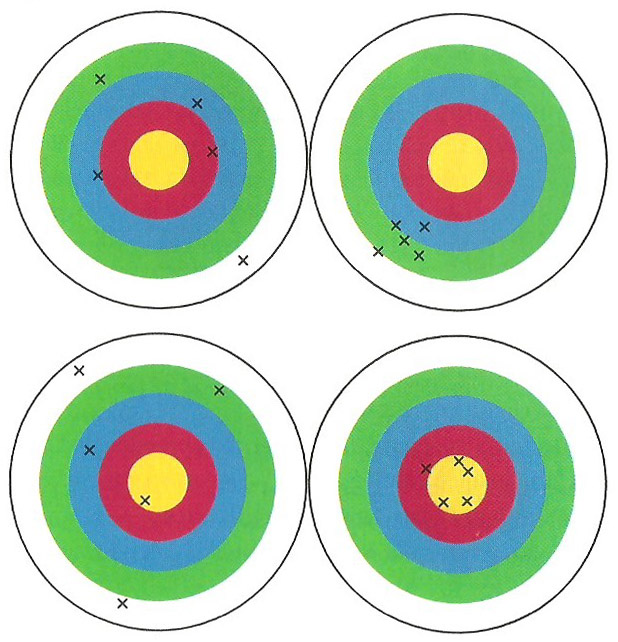
\includegraphics[scale=0.8]{stat-32.jpg}
\end{center}

Pour chaque tireur, on considère la distance de chaque flèche au centre de la cible.
\begin{enumerate}
\item Associer chaque couple (moyenne;écart-type) à chaque cible : (2,84;0,97); (0,79;0,19); (3,33;0,55); (3,21;1,42).
\item Associer chacun des tireurs à une cible : Un tireur expérimenté, deux débutants et un tireur expérimenté qui a mal réglé son viseur.
\end{enumerate} 